% Options for packages loaded elsewhere
\PassOptionsToPackage{unicode}{hyperref}
\PassOptionsToPackage{hyphens}{url}
%
\documentclass[
  ,man,floatsintext]{apa6}
\usepackage{amsmath,amssymb}
\usepackage{iftex}
\ifPDFTeX
  \usepackage[T1]{fontenc}
  \usepackage[utf8]{inputenc}
  \usepackage{textcomp} % provide euro and other symbols
\else % if luatex or xetex
  \usepackage{unicode-math} % this also loads fontspec
  \defaultfontfeatures{Scale=MatchLowercase}
  \defaultfontfeatures[\rmfamily]{Ligatures=TeX,Scale=1}
\fi
\usepackage{lmodern}
\ifPDFTeX\else
  % xetex/luatex font selection
\fi
% Use upquote if available, for straight quotes in verbatim environments
\IfFileExists{upquote.sty}{\usepackage{upquote}}{}
\IfFileExists{microtype.sty}{% use microtype if available
  \usepackage[]{microtype}
  \UseMicrotypeSet[protrusion]{basicmath} % disable protrusion for tt fonts
}{}
\makeatletter
\@ifundefined{KOMAClassName}{% if non-KOMA class
  \IfFileExists{parskip.sty}{%
    \usepackage{parskip}
  }{% else
    \setlength{\parindent}{0pt}
    \setlength{\parskip}{6pt plus 2pt minus 1pt}}
}{% if KOMA class
  \KOMAoptions{parskip=half}}
\makeatother
\usepackage{xcolor}
\usepackage{color}
\usepackage{fancyvrb}
\newcommand{\VerbBar}{|}
\newcommand{\VERB}{\Verb[commandchars=\\\{\}]}
\DefineVerbatimEnvironment{Highlighting}{Verbatim}{commandchars=\\\{\}}
% Add ',fontsize=\small' for more characters per line
\usepackage{framed}
\definecolor{shadecolor}{RGB}{248,248,248}
\newenvironment{Shaded}{\begin{snugshade}}{\end{snugshade}}
\newcommand{\AlertTok}[1]{\textcolor[rgb]{0.94,0.16,0.16}{#1}}
\newcommand{\AnnotationTok}[1]{\textcolor[rgb]{0.56,0.35,0.01}{\textbf{\textit{#1}}}}
\newcommand{\AttributeTok}[1]{\textcolor[rgb]{0.13,0.29,0.53}{#1}}
\newcommand{\BaseNTok}[1]{\textcolor[rgb]{0.00,0.00,0.81}{#1}}
\newcommand{\BuiltInTok}[1]{#1}
\newcommand{\CharTok}[1]{\textcolor[rgb]{0.31,0.60,0.02}{#1}}
\newcommand{\CommentTok}[1]{\textcolor[rgb]{0.56,0.35,0.01}{\textit{#1}}}
\newcommand{\CommentVarTok}[1]{\textcolor[rgb]{0.56,0.35,0.01}{\textbf{\textit{#1}}}}
\newcommand{\ConstantTok}[1]{\textcolor[rgb]{0.56,0.35,0.01}{#1}}
\newcommand{\ControlFlowTok}[1]{\textcolor[rgb]{0.13,0.29,0.53}{\textbf{#1}}}
\newcommand{\DataTypeTok}[1]{\textcolor[rgb]{0.13,0.29,0.53}{#1}}
\newcommand{\DecValTok}[1]{\textcolor[rgb]{0.00,0.00,0.81}{#1}}
\newcommand{\DocumentationTok}[1]{\textcolor[rgb]{0.56,0.35,0.01}{\textbf{\textit{#1}}}}
\newcommand{\ErrorTok}[1]{\textcolor[rgb]{0.64,0.00,0.00}{\textbf{#1}}}
\newcommand{\ExtensionTok}[1]{#1}
\newcommand{\FloatTok}[1]{\textcolor[rgb]{0.00,0.00,0.81}{#1}}
\newcommand{\FunctionTok}[1]{\textcolor[rgb]{0.13,0.29,0.53}{\textbf{#1}}}
\newcommand{\ImportTok}[1]{#1}
\newcommand{\InformationTok}[1]{\textcolor[rgb]{0.56,0.35,0.01}{\textbf{\textit{#1}}}}
\newcommand{\KeywordTok}[1]{\textcolor[rgb]{0.13,0.29,0.53}{\textbf{#1}}}
\newcommand{\NormalTok}[1]{#1}
\newcommand{\OperatorTok}[1]{\textcolor[rgb]{0.81,0.36,0.00}{\textbf{#1}}}
\newcommand{\OtherTok}[1]{\textcolor[rgb]{0.56,0.35,0.01}{#1}}
\newcommand{\PreprocessorTok}[1]{\textcolor[rgb]{0.56,0.35,0.01}{\textit{#1}}}
\newcommand{\RegionMarkerTok}[1]{#1}
\newcommand{\SpecialCharTok}[1]{\textcolor[rgb]{0.81,0.36,0.00}{\textbf{#1}}}
\newcommand{\SpecialStringTok}[1]{\textcolor[rgb]{0.31,0.60,0.02}{#1}}
\newcommand{\StringTok}[1]{\textcolor[rgb]{0.31,0.60,0.02}{#1}}
\newcommand{\VariableTok}[1]{\textcolor[rgb]{0.00,0.00,0.00}{#1}}
\newcommand{\VerbatimStringTok}[1]{\textcolor[rgb]{0.31,0.60,0.02}{#1}}
\newcommand{\WarningTok}[1]{\textcolor[rgb]{0.56,0.35,0.01}{\textbf{\textit{#1}}}}
\usepackage{graphicx}
\makeatletter
\def\maxwidth{\ifdim\Gin@nat@width>\linewidth\linewidth\else\Gin@nat@width\fi}
\def\maxheight{\ifdim\Gin@nat@height>\textheight\textheight\else\Gin@nat@height\fi}
\makeatother
% Scale images if necessary, so that they will not overflow the page
% margins by default, and it is still possible to overwrite the defaults
% using explicit options in \includegraphics[width, height, ...]{}
\setkeys{Gin}{width=\maxwidth,height=\maxheight,keepaspectratio}
% Set default figure placement to htbp
\makeatletter
\def\fps@figure{htbp}
\makeatother
\setlength{\emergencystretch}{3em} % prevent overfull lines
\providecommand{\tightlist}{%
  \setlength{\itemsep}{0pt}\setlength{\parskip}{0pt}}
\setcounter{secnumdepth}{-\maxdimen} % remove section numbering
% Make \paragraph and \subparagraph free-standing
\makeatletter
\ifx\paragraph\undefined\else
  \let\oldparagraph\paragraph
  \renewcommand{\paragraph}{
    \@ifstar
      \xxxParagraphStar
      \xxxParagraphNoStar
  }
  \newcommand{\xxxParagraphStar}[1]{\oldparagraph*{#1}\mbox{}}
  \newcommand{\xxxParagraphNoStar}[1]{\oldparagraph{#1}\mbox{}}
\fi
\ifx\subparagraph\undefined\else
  \let\oldsubparagraph\subparagraph
  \renewcommand{\subparagraph}{
    \@ifstar
      \xxxSubParagraphStar
      \xxxSubParagraphNoStar
  }
  \newcommand{\xxxSubParagraphStar}[1]{\oldsubparagraph*{#1}\mbox{}}
  \newcommand{\xxxSubParagraphNoStar}[1]{\oldsubparagraph{#1}\mbox{}}
\fi
\makeatother
\ifLuaTeX
\usepackage[bidi=basic]{babel}
\else
\usepackage[bidi=default]{babel}
\fi
\babelprovide[main,import]{english}
% get rid of language-specific shorthands (see #6817):
\let\LanguageShortHands\languageshorthands
\def\languageshorthands#1{}
% Manuscript styling
\usepackage{upgreek}
\captionsetup{font=singlespacing,justification=justified}

% Table formatting
\usepackage{longtable}
\usepackage{lscape}
% \usepackage[counterclockwise]{rotating}   % Landscape page setup for large tables
\usepackage{multirow}		% Table styling
\usepackage{tabularx}		% Control Column width
\usepackage[flushleft]{threeparttable}	% Allows for three part tables with a specified notes section
\usepackage{threeparttablex}            % Lets threeparttable work with longtable

% Create new environments so endfloat can handle them
% \newenvironment{ltable}
%   {\begin{landscape}\centering\begin{threeparttable}}
%   {\end{threeparttable}\end{landscape}}
\newenvironment{lltable}{\begin{landscape}\centering\begin{ThreePartTable}}{\end{ThreePartTable}\end{landscape}}

% Enables adjusting longtable caption width to table width
% Solution found at http://golatex.de/longtable-mit-caption-so-breit-wie-die-tabelle-t15767.html
\makeatletter
\newcommand\LastLTentrywidth{1em}
\newlength\longtablewidth
\setlength{\longtablewidth}{1in}
\newcommand{\getlongtablewidth}{\begingroup \ifcsname LT@\roman{LT@tables}\endcsname \global\longtablewidth=0pt \renewcommand{\LT@entry}[2]{\global\advance\longtablewidth by ##2\relax\gdef\LastLTentrywidth{##2}}\@nameuse{LT@\roman{LT@tables}} \fi \endgroup}

% \setlength{\parindent}{0.5in}
% \setlength{\parskip}{0pt plus 0pt minus 0pt}

% Overwrite redefinition of paragraph and subparagraph by the default LaTeX template
% See https://github.com/crsh/papaja/issues/292
\makeatletter
\renewcommand{\paragraph}{\@startsection{paragraph}{4}{\parindent}%
  {0\baselineskip \@plus 0.2ex \@minus 0.2ex}%
  {-1em}%
  {\normalfont\normalsize\bfseries\itshape\typesectitle}}

\renewcommand{\subparagraph}[1]{\@startsection{subparagraph}{5}{1em}%
  {0\baselineskip \@plus 0.2ex \@minus 0.2ex}%
  {-\z@\relax}%
  {\normalfont\normalsize\itshape\hspace{\parindent}{#1}\textit{\addperi}}{\relax}}
\makeatother

\makeatletter
\usepackage{etoolbox}
\patchcmd{\maketitle}
  {\section{\normalfont\normalsize\abstractname}}
  {\section*{\normalfont\normalsize\abstractname}}
  {}{\typeout{Failed to patch abstract.}}
\patchcmd{\maketitle}
  {\section{\protect\normalfont{\@title}}}
  {\section*{\protect\normalfont{\@title}}}
  {}{\typeout{Failed to patch title.}}
\makeatother

\usepackage{xpatch}
\makeatletter
\xapptocmd\appendix
  {\xapptocmd\section
    {\addcontentsline{toc}{section}{\appendixname\ifoneappendix\else~\theappendix\fi: #1}}
    {}{\InnerPatchFailed}%
  }
{}{\PatchFailed}
\makeatother
\keywords{keywords\newline\indent Word count: X}
\usepackage{csquotes}
\usepackage[titles]{tocloft}
\cftpagenumbersoff{figure}
\renewcommand{\cftfigpresnum}{\itshape\figurename\enspace}
\renewcommand{\cftfigaftersnum}{.\space}
\setlength{\cftfigindent}{0pt}
\setlength{\cftafterloftitleskip}{0pt}
\settowidth{\cftfignumwidth}{Figure 10.\qquad}
\cftpagenumbersoff{table}
\renewcommand{\cfttabpresnum}{\itshape\tablename\enspace}
\renewcommand{\cfttabaftersnum}{.\space}
\setlength{\cfttabindent}{0pt}
\setlength{\cftafterloftitleskip}{0pt}
\settowidth{\cfttabnumwidth}{Table 10.\qquad}
\ifLuaTeX
  \usepackage{selnolig}  % disable illegal ligatures
\fi
\usepackage{bookmark}
\IfFileExists{xurl.sty}{\usepackage{xurl}}{} % add URL line breaks if available
\urlstyle{same}
\hypersetup{
  pdftitle={Variation of {[}v{]} in Cook Islands Māori},
  pdfauthor={Quartz ColvinRutgers University},
  pdflang={en-EN},
  pdfkeywords={keywords},
  hidelinks,
  pdfcreator={LaTeX via pandoc}}

\title{Variation of {[}v{]} in Cook Islands Māori}
\author{Quartz Colvin\textsuperscript{Rutgers University}}
\date{}


\shorttitle{Cook Islands Māori}

\affiliation{\phantom{0}}

\begin{document}
\maketitle

\section{1.0 Introduction}\label{introduction}

In this paper, we will do a statistical analysis of {[}v{]} across a sample of islands in Cook Islands Māori (CIM). It is known that in many dialects and other varieties of Māori, this phoneme can be realized as {[}w{]} or {[}v{]}. This paper aims to take a statistical approach to this generalization.

This paper has four sub-questions to investigate. First, how does w\textasciitilde v duration vary by island and second, how does intensity for these phonemes vary by island. The other two questions are about identifying information about the surface forms of w\textasciitilde v by island. Specifically, we will model f0 and f2 to determine whether certain islands have a voiced phoneme realized. Finally, the f2 model will help us determine which islands have higher rates of {[}w{]}s surfacing and which have more {[}v{]}s surfacing.

\subsection{1.1 Background (CIM)}\label{background-cim}

Cook Islands Māori is an Eastern Polynesian language classified as \emph{Endangered}. It is very closely related to Aotearoa Māori, but is definitely different from it.

It is known across both Aotearoa (NZ) Māori and CIM that some speakers regularly pronounce {[}v{]} as {[}w{]}, but it is not clear to anyone who does this more and what conditions it.

\textbf{???fill in}

\section{2.0 Methods}\label{methods}

\textbf{???fill in}

\section{3.0 Data}\label{data}

The following large data set has many columns. Here I show a preview of the data set and then discuss which columns will be relevant to the analysis later in the paper.

\begin{Shaded}
\begin{Highlighting}[]
\NormalTok{knitr}\SpecialCharTok{::}\FunctionTok{kable}\NormalTok{(}\FunctionTok{head}\NormalTok{(untidy\_data))}
\end{Highlighting}
\end{Shaded}

\begin{tabular}{l|l|l|l|l|l|l|r|r|r|r|r|r|r|r|r|r}
\hline
speaker & island & Filename & TextGridLabel & Word & PreviousLabel & FollowingLabel & start & end & duration & f0\_20.point & f0\_50.point & f0\_80.point & F1\_midpoint & F2\_midpoint & F3\_midpoint & intensity\_midpoint\\
\hline
AAN & Rarotonga & AAN-RRAAT8-018 & a & rave & r & v & 1.10 & 1.13 & 0.03 & 144.0532 & 143.0606 & 141.8219 & 356.4547 & 1755.623 & 2797.351 & 40.29265\\
\hline
AAN & Rarotonga & AAN-RRAAT8-018 & v & rave & a & e & 1.13 & 1.16 & 0.03 & 141.7901 & 142.2725 & 143.3506 & 335.4101 & 1999.837 & 3192.717 & 39.22013\\
\hline
AAN & Rarotonga & AAN-RRAAT8-018 & e & rave & v & NA & 1.16 & 1.19 & 0.03 & 143.1055 & 142.6605 & 142.2108 & 341.6010 & 2362.305 & 3280.530 & 40.47651\\
\hline
AAN & Rarotonga & AAN-RRAAT8-052 & v & vaꞌine & NA & a & 1.73 & 1.76 & 0.03 & 263.7962 & 269.8593 & 270.8541 & 537.7380 & 1040.550 & 2898.961 & 52.75762\\
\hline
AAN & Rarotonga & AAN-RRAAT8-052 & a & vaꞌine & v & ꞌ & 1.76 & 1.79 & 0.03 & 265.8672 & 261.0071 & 263.7023 & 584.4075 & 1419.937 & 2876.166 & 55.72719\\
\hline
AAN & Rarotonga & AAN-RRAAT8-060 & a & rava & r & v & 0.75 & 0.80 & 0.05 & 203.7388 & 202.9822 & 201.2384 & 670.0677 & 1474.651 & 2556.541 & 52.94500\\
\hline
\end{tabular}

First, note that there is no `id' column but there is a column for the speaker's initials. I will use speaker in place of `id' because that is what was in this original data set. The `island' column states what island that speaker is from. This data only contains data from the four islands Atiu, Mauke, Penrhyn and Rarotonga. Duration corresponds to the total duration of the phoneme, and intensity is measured at the midpoint of the phoneme.

F0 values were taken at 20\%, 50\% and 80\% of each phoneme's total duration. Later, we will opt to use only the F0 values at 50\%, but that will be discussed more later. Finally, F2\_midpoint is f2 measured in Hz at the midpoint of that phoneme.

All of the other columns are either straight forward information or will be irrelevant for this paper.

\section{4.0 Analysis}\label{analysis}

This section readdresses the main questions about the w\textasciitilde v alternation. First, how does duration differ by island and second, how does intensity vary by island? Finally, do any islands have regular occurrence of {[}w{]} instead of {[}v{]} surfacing. For this final question, we will compare f0 and f2 separately.

Note that in all of my models, I did not control for where w\textasciitilde v occurs in the word, since I am looking at general frequency information and not doing a phonological analysis of specific environments in which {[}w{]} or {[}v{]} occurs more. Another important thing to note is that for each island, there were different numbers of speakers contributing to the data set. All of the Atiu data came from one speaker and it was the same for Penrhyn. The Mauke data came from four speakers and the Rarotonga data came from five speakers.

Since there are different numbers of speakers from each of these islands, the models I will use to investigate each question will be linear mixed models.

\subsection{4.1 Duration by island}\label{duration-by-island}

The first step of comparing duration of w\textasciitilde v across these four islands is to make a smaller, tidy data set that only contains the relevant information.

Below, I filter the data so that it only contains rows with the ``v'' phoneme. Then I arrange it by island and then by word, and I select only the columns ``speaker'', ``island'', ``word'' and duration. Finally, I save this filtered data set as a new csv file.

\begin{Shaded}
\begin{Highlighting}[]
\NormalTok{tidy\_dur }\OtherTok{\textless{}{-}}\NormalTok{ untidy\_data }\SpecialCharTok{|\textgreater{}}
  \FunctionTok{filter}\NormalTok{(TextGridLabel }\SpecialCharTok{==} \StringTok{"v"}\NormalTok{) }\SpecialCharTok{|\textgreater{}}  
  \FunctionTok{arrange}\NormalTok{(island, Word) }\SpecialCharTok{|\textgreater{}}  
  \FunctionTok{select}\NormalTok{(speaker, island, }\AttributeTok{word =}\NormalTok{ Word, duration) }\SpecialCharTok{|\textgreater{}}
  \FunctionTok{write\_csv}\NormalTok{(}\FunctionTok{here}\NormalTok{(}\StringTok{"tidy\_data"}\NormalTok{, }\StringTok{"tidy\_dur.csv"}\NormalTok{))}
\end{Highlighting}
\end{Shaded}

After we have done this tidying process, the duration data set looks like this.

\begin{tabular}{l|l|l|r}
\hline
speaker & island & word & duration\\
\hline
TA & Atiu & ava & 0.08\\
\hline
TA & Atiu & ava & 0.07\\
\hline
TA & Atiu & ava & 0.14\\
\hline
TA & Atiu & ava & 0.11\\
\hline
TA & Atiu & ava & 0.05\\
\hline
TA & Atiu & ava & 0.13\\
\hline
\end{tabular}

For a visual comparison, we will look at boxplots comparing duration across these four islands. The code chunk for the box plot is here and the actual plot is below it.

\begin{Shaded}
\begin{Highlighting}[]
\NormalTok{plot\_dur }\OtherTok{\textless{}{-}}\NormalTok{ tidy\_dur }\SpecialCharTok{|\textgreater{}}
  \FunctionTok{ggplot}\NormalTok{() }\SpecialCharTok{+}
  \FunctionTok{aes}\NormalTok{(}\AttributeTok{x =}\NormalTok{ island, }\AttributeTok{y =}\NormalTok{ duration, }\AttributeTok{color =}\NormalTok{ island) }\SpecialCharTok{+}
  \FunctionTok{geom\_boxplot}\NormalTok{() }\SpecialCharTok{+}
  \FunctionTok{labs}\NormalTok{(}
    \AttributeTok{title =} \StringTok{"Compare [v] duration by island"}\NormalTok{,}
    \AttributeTok{x =} \StringTok{"Island"}\NormalTok{,}
    \AttributeTok{y =} \StringTok{"Duration"}
\NormalTok{  )}
\end{Highlighting}
\end{Shaded}

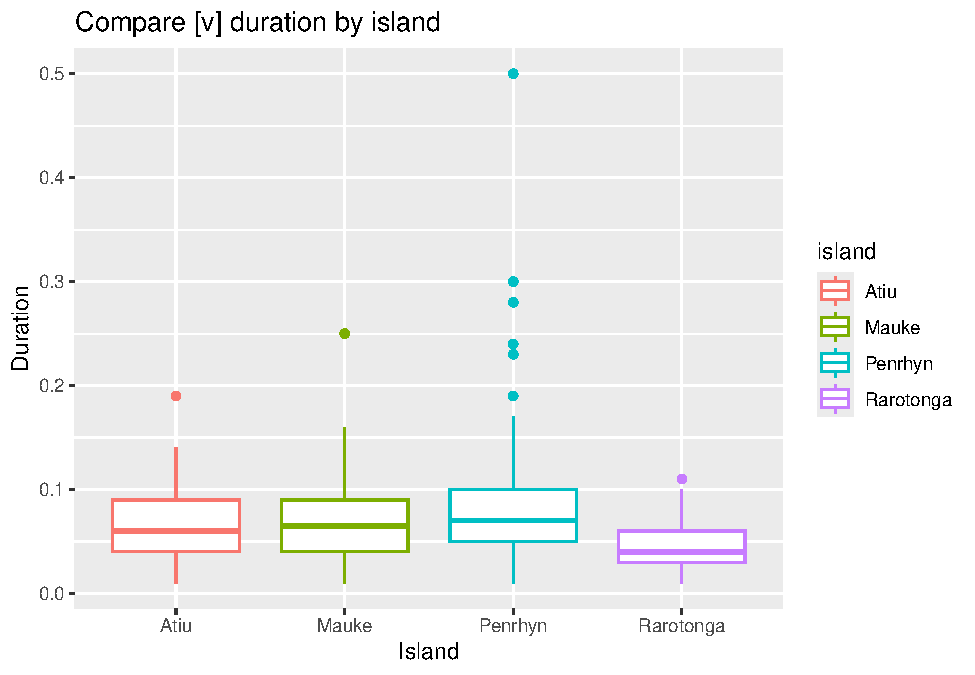
\includegraphics{D2_CIM_files/figure-latex/print-duration-plot-1.pdf}

The boxplot shows that average (mean) durations were pretty similar across these three islands. But for some reason, Penrhyn had a much larger range of durations than the other islands.

Now that we have an idea of what the general differences and similarities are for duration, we can fit the linear mixed effect model. In the code chunk. you can see that I account for the fact that number of speakers varies across the islands in the data set, and also that there are many instances of each word. These instances of each `word' are repeated by each speaker multiple times and by several speakers multiple times.

\begin{Shaded}
\begin{Highlighting}[]
\NormalTok{mod\_dur }\OtherTok{\textless{}{-}} \FunctionTok{lmer}\NormalTok{(duration }\SpecialCharTok{\textasciitilde{}}\NormalTok{ island }\SpecialCharTok{+}\NormalTok{ (}\DecValTok{1}\SpecialCharTok{|}\NormalTok{speaker) }\SpecialCharTok{+}\NormalTok{ (}\DecValTok{1}\SpecialCharTok{|}\NormalTok{word), }\AttributeTok{data =}\NormalTok{ tidy\_dur)}
\end{Highlighting}
\end{Shaded}

\begin{verbatim}
## Linear mixed model fit by REML. t-tests use Satterthwaite's method [
## lmerModLmerTest]
## Formula: duration ~ island + (1 | speaker) + (1 | word)
##    Data: tidy_dur
## 
## REML criterion at convergence: -3416.3
## 
## Scaled residuals: 
##     Min      1Q  Median      3Q     Max 
## -2.8215 -0.5539 -0.0851  0.4095  7.5763 
## 
## Random effects:
##  Groups   Name        Variance  Std.Dev.
##  word     (Intercept) 0.0007328 0.02707 
##  speaker  (Intercept) 0.0001517 0.01231 
##  Residual             0.0010189 0.03192 
## Number of obs: 896, groups:  word, 145; speaker, 11
## 
## Fixed effects:
##                  Estimate Std. Error        df t value Pr(>|t|)   
## (Intercept)      0.064761   0.013130  6.339137   4.932  0.00225 **
## islandMauke     -0.001702   0.014390  5.858906  -0.118  0.90982   
## islandPenrhyn    0.019477   0.018068  5.690570   1.078  0.32459   
## islandRarotonga -0.018439   0.014557  6.292463  -1.267  0.25014   
## ---
## Signif. codes:  0 '***' 0.001 '**' 0.01 '*' 0.05 '.' 0.1 ' ' 1
## 
## Correlation of Fixed Effects:
##             (Intr) islndM islndP
## islandMauke -0.876              
## islndPnrhyn -0.698  0.637       
## islandRrtng -0.869  0.793  0.632
\end{verbatim}

The p-values for each island are as follows. Atiu's p-value = 0.00225, Mauke's p-value = 0.90982, Penrhyn's p-value = 0.32459, and Rarotonga's p-value = 0.25014.

\subsection{4.2 Intensity by island}\label{intensity-by-island}

Next is the intensity comparison across the four islands. Starting from the raw data set, we must filter it again so that it only has instances of the ``v'' phoneme and we filter everything except the ``speaker'', ``island'', ``word'', and ``intensity'' columns. The tidying process is shown in the code chunk here.

\begin{Shaded}
\begin{Highlighting}[]
\NormalTok{tidy\_intense }\OtherTok{\textless{}{-}}\NormalTok{ untidy\_data }\SpecialCharTok{|\textgreater{}}
  \FunctionTok{filter}\NormalTok{(TextGridLabel }\SpecialCharTok{==} \StringTok{"v"}\NormalTok{) }\SpecialCharTok{|\textgreater{}}  
  \FunctionTok{arrange}\NormalTok{(island, Word) }\SpecialCharTok{|\textgreater{}}  
  \FunctionTok{select}\NormalTok{(speaker, island, }\AttributeTok{word =}\NormalTok{ Word, }\AttributeTok{intensity =}\NormalTok{ intensity\_midpoint) }\SpecialCharTok{|\textgreater{}}
  \FunctionTok{write\_csv}\NormalTok{(}\FunctionTok{here}\NormalTok{(}\StringTok{"tidy\_data"}\NormalTok{, }\StringTok{"tidy\_intense.csv"}\NormalTok{))}
\end{Highlighting}
\end{Shaded}

Once the new data set has been made, it looks roughly like the following table, but extended of course.

\begin{tabular}{l|l|l|r}
\hline
speaker & island & word & intensity\\
\hline
TA & Atiu & ava & 54.08202\\
\hline
TA & Atiu & ava & 58.06061\\
\hline
TA & Atiu & ava & 48.40481\\
\hline
TA & Atiu & ava & 54.18315\\
\hline
TA & Atiu & ava & 49.59224\\
\hline
TA & Atiu & ava & 53.07335\\
\hline
\end{tabular}

In the same way we did for the duration question, we will first look at a boxplot to visually see any clear differences in intensity across the Cook Islands. The code chunk to make the plot is below, and then the actual plot is printed below it.

\begin{Shaded}
\begin{Highlighting}[]
\NormalTok{plot\_intense }\OtherTok{\textless{}{-}}\NormalTok{ tidy\_intense }\SpecialCharTok{|\textgreater{}}
  \FunctionTok{ggplot}\NormalTok{() }\SpecialCharTok{+}
  \FunctionTok{aes}\NormalTok{(}\AttributeTok{x =}\NormalTok{ island, }\AttributeTok{y =}\NormalTok{ intensity, }\AttributeTok{color =}\NormalTok{ island) }\SpecialCharTok{+}
  \FunctionTok{geom\_boxplot}\NormalTok{() }\SpecialCharTok{+}
  \FunctionTok{labs}\NormalTok{(}
    \AttributeTok{title =} \StringTok{"Compare [v] intensity by island"}\NormalTok{,}
    \AttributeTok{x =} \StringTok{"Island"}\NormalTok{,}
    \AttributeTok{y =} \StringTok{"Intensity"}
\NormalTok{  ) }
\end{Highlighting}
\end{Shaded}

\begin{figure}
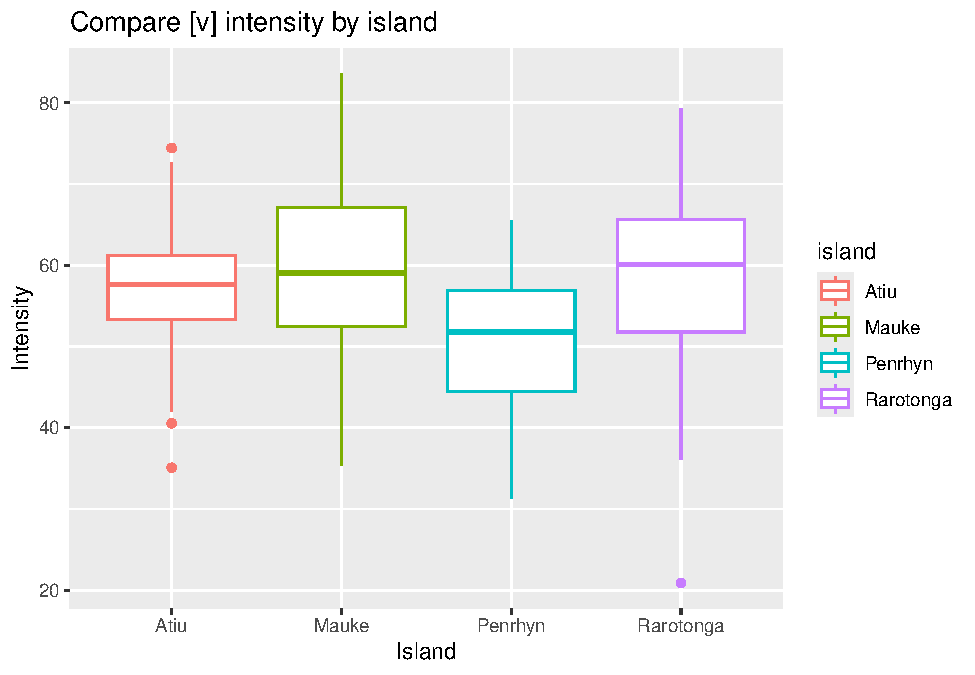
\includegraphics[width=1500px]{D2_CIM_files/figure-latex/print-intensity-plot-1} \caption{ }\label{fig:print-intensity-plot}
\end{figure}

Initially, it is clear that Penrhyn has the lowest mean intensity for w\textasciitilde v. Mauke and Rarotonga have nearly the same mean intensity, and Atiu's mean is slighly lower, but not as low as Penrhyn's mean.

Now that we know the general patterns, we can fit our linear mixed effects model. Dur to the same reasons as before, I model speaker and word as mixed effects in the intensity by island model. The code chunk below shows how I fit the model in R.

\begin{Shaded}
\begin{Highlighting}[]
\NormalTok{mod\_intense }\OtherTok{\textless{}{-}} \FunctionTok{lmer}\NormalTok{(intensity }\SpecialCharTok{\textasciitilde{}}\NormalTok{ island }\SpecialCharTok{+}\NormalTok{ (}\DecValTok{1}\SpecialCharTok{|}\NormalTok{speaker) }\SpecialCharTok{+}\NormalTok{ (}\DecValTok{1}\SpecialCharTok{|}\NormalTok{word), }\AttributeTok{data =}\NormalTok{ tidy\_intense)}
\end{Highlighting}
\end{Shaded}

The p-values for each island are as follows. Atiu's p-value = 0.00161, Mauke's p-value = 0.84133, Penrhyn's p-value = 0.62670 and Rarotonga's p-value = 0.86632.

\begin{verbatim}
## Linear mixed model fit by REML. t-tests use Satterthwaite's method [
## lmerModLmerTest]
## Formula: intensity ~ island + (1 | speaker) + (1 | word)
##    Data: tidy_intense
## 
## REML criterion at convergence: 5865.9
## 
## Scaled residuals: 
##     Min      1Q  Median      3Q     Max 
## -4.2068 -0.5148  0.1031  0.5991  2.5860 
## 
## Random effects:
##  Groups   Name        Variance Std.Dev.
##  word     (Intercept)  19.16    4.377  
##  speaker  (Intercept) 117.38   10.834  
##  Residual              34.24    5.851  
## Number of obs: 894, groups:  word, 145; speaker, 11
## 
## Fixed effects:
##                 Estimate Std. Error     df t value Pr(>|t|)   
## (Intercept)       57.919     10.864  6.184   5.331  0.00161 **
## islandMauke        2.534     12.137  6.165   0.209  0.84133   
## islandPenrhyn     -7.853     15.347  6.156  -0.512  0.62670   
## islandRarotonga    2.095     11.947  6.261   0.175  0.86632   
## ---
## Signif. codes:  0 '***' 0.001 '**' 0.01 '*' 0.05 '.' 0.1 ' ' 1
## 
## Correlation of Fixed Effects:
##             (Intr) islndM islndP
## islandMauke -0.894              
## islndPnrhyn -0.707  0.633       
## islandRrtng -0.908  0.813  0.643
\end{verbatim}

\subsection{4.3 Voicing by island}\label{voicing-by-island}

Moving on to the formant questions, first we will investigate how voicing of w\textasciitilde v differs across these four islands.

This time, we tidy the raw data set in a similar way but with one additional step. Since we have f0 values at three different intervals of the same morpheme, if we were to put all of those formant values in a new column and the percentage in another new column, then it would fabricate 3 times as many tokens that were not elicited from the speakers.

In order to limit this autocorrelation issue, I chose to only keep f0 values at the 50\% interval of the phoneme. I chose the 50\% interval because the middle of the duration seemed like the smartest choice to represent the average f0 value across the phoneme's duration.

The code chunk below shows how I tidied this mini-data-set to answer the voicing question.

\begin{Shaded}
\begin{Highlighting}[]
\NormalTok{tidy\_f0 }\OtherTok{\textless{}{-}}\NormalTok{ untidy\_data }\SpecialCharTok{|\textgreater{}}
  \FunctionTok{filter}\NormalTok{(TextGridLabel }\SpecialCharTok{==} \StringTok{"v"}\NormalTok{) }\SpecialCharTok{|\textgreater{}}
  \FunctionTok{pivot\_longer}\NormalTok{(}
    \AttributeTok{cols =} \FunctionTok{c}\NormalTok{(}\StringTok{"f0\_50.point"}\NormalTok{), }
    \AttributeTok{names\_to =} \StringTok{"percent"}\NormalTok{,}
    \AttributeTok{values\_to =} \StringTok{"f0"}
\NormalTok{  ) }\SpecialCharTok{|\textgreater{}}
  \FunctionTok{arrange}\NormalTok{(island, Word) }\SpecialCharTok{|\textgreater{}}  
  \FunctionTok{select}\NormalTok{(speaker, island, }\AttributeTok{word =}\NormalTok{ Word, f0, duration) }\SpecialCharTok{|\textgreater{}}
  \FunctionTok{write\_csv}\NormalTok{(}\FunctionTok{here}\NormalTok{(}\StringTok{"tidy\_data"}\NormalTok{, }\StringTok{"tidy\_f0.csv"}\NormalTok{))}
\end{Highlighting}
\end{Shaded}

Once we have made this new, tidy data set, it looks like this. Again, if I showed the full table, it would have more than this one word and this one island. This is just the top few rows of the sorted table.

\begin{tabular}{l|l|l|r|r}
\hline
speaker & island & word & f0 & duration\\
\hline
TA & Atiu & ava & 127.0908 & 0.08\\
\hline
TA & Atiu & ava & 157.4397 & 0.07\\
\hline
TA & Atiu & ava & 134.1155 & 0.14\\
\hline
TA & Atiu & ava & 141.8125 & 0.11\\
\hline
TA & Atiu & ava & 118.2318 & 0.05\\
\hline
TA & Atiu & ava & 142.7506 & 0.13\\
\hline
\end{tabular}

This time, to compare f0 across the islands visually, we can plot this data onto a scatterplot. First, here is the code chunk to create the scatterplots.

\begin{Shaded}
\begin{Highlighting}[]
\NormalTok{f0\_plot }\OtherTok{\textless{}{-}}\NormalTok{ tidy\_f0 }\SpecialCharTok{|\textgreater{}}
  \FunctionTok{ggplot}\NormalTok{() }\SpecialCharTok{+} 
  \FunctionTok{aes}\NormalTok{(}\AttributeTok{x =}\NormalTok{ duration, }\AttributeTok{y =}\NormalTok{ f0, }\AttributeTok{color =}\NormalTok{ speaker) }\SpecialCharTok{+}
  \FunctionTok{geom\_point}\NormalTok{() }\SpecialCharTok{+}
  \FunctionTok{geom\_smooth}\NormalTok{(}
    \AttributeTok{method=}\StringTok{"glm"}\NormalTok{,}
    \AttributeTok{color=}\StringTok{"black"}\NormalTok{,}
    \AttributeTok{method.args =} \FunctionTok{list}\NormalTok{(}\AttributeTok{family =} \StringTok{"poisson"}\NormalTok{)}
\NormalTok{  ) }\SpecialCharTok{+}
  \FunctionTok{facet\_grid}\NormalTok{(.}\SpecialCharTok{\textasciitilde{}}\NormalTok{island,}
             \AttributeTok{scales =} \StringTok{"free\_x"}\NormalTok{) }\SpecialCharTok{+}
  \FunctionTok{labs}\NormalTok{(}
    \AttributeTok{title =} \StringTok{"Compare F0 across islands"}\NormalTok{, }
    \AttributeTok{x =} \StringTok{"Duration"}\NormalTok{, }
    \AttributeTok{y =} \StringTok{"F0 (Hz)"}
\NormalTok{  ) }
\end{Highlighting}
\end{Shaded}

As you can see, I created an individual facet for each island and each color represents data from a particular speaker.

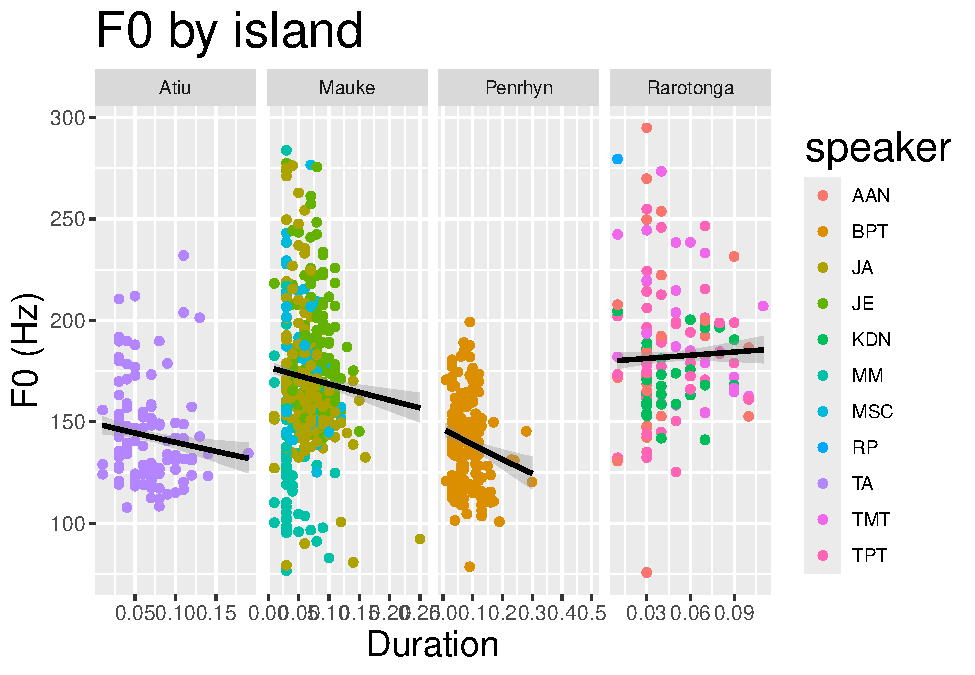
\includegraphics{D2_CIM_files/figure-latex/print-f0-plot-1.pdf}

It's clear that the most drastic slope is in the Penrhyn plot, and the data for the islands with more speakers are much more spread out across the plot.

To formally compare these different variables, we can again use a linear mixed effects model to see how f0 varies across these four Cook Islands. The model fitting is shown in the code chunk below.

\begin{Shaded}
\begin{Highlighting}[]
\NormalTok{mod\_f0 }\OtherTok{\textless{}{-}} \FunctionTok{lmer}\NormalTok{(f0 }\SpecialCharTok{\textasciitilde{}}\NormalTok{ island }\SpecialCharTok{+}\NormalTok{ (}\DecValTok{1}\SpecialCharTok{|}\NormalTok{speaker) }\SpecialCharTok{+}\NormalTok{ (}\DecValTok{1}\SpecialCharTok{|}\NormalTok{word), }\AttributeTok{data =}\NormalTok{ tidy\_f0)}
\end{Highlighting}
\end{Shaded}

The p-values for each island in this model are as follows. Atiu's p-value = 0.00702, Mauke's p-value = 0.43464, Penrhyn's p-value is 0.93276, and Rarotonga's p-value = 0.14965.

\begin{verbatim}
## Linear mixed model fit by REML. t-tests use Satterthwaite's method [
## lmerModLmerTest]
## Formula: f0 ~ island + (1 | speaker) + (1 | word)
##    Data: tidy_f0
## 
## REML criterion at convergence: 8097.3
## 
## Scaled residuals: 
##     Min      1Q  Median      3Q     Max 
## -3.8763 -0.6582 -0.1477  0.5171  5.0606 
## 
## Random effects:
##  Groups   Name        Variance Std.Dev.
##  word     (Intercept) 130.1    11.41   
##  speaker  (Intercept) 592.5    24.34   
##  Residual             822.2    28.67   
## Number of obs: 841, groups:  word, 134; speaker, 11
## 
## Fixed effects:
##                 Estimate Std. Error      df t value Pr(>|t|)   
## (Intercept)      140.935     24.584   3.466   5.733  0.00702 **
## islandMauke       24.229     27.450   3.448   0.883  0.43464   
## islandPenrhyn     -3.145     34.660   3.423  -0.091  0.93276   
## islandRarotonga   49.950     27.269   3.564   1.832  0.14965   
## ---
## Signif. codes:  0 '***' 0.001 '**' 0.01 '*' 0.05 '.' 0.1 ' ' 1
## 
## Correlation of Fixed Effects:
##             (Intr) islndM islndP
## islandMauke -0.893              
## islndPnrhyn -0.707  0.633       
## islandRrtng -0.899  0.805  0.638
\end{verbatim}

\subsection{4.4 w\textasciitilde v distribution by island}\label{wv-distribution-by-island}

Finally we turn to the main research question: is there a correlation between island and how many {[}w{]} tokens surface?

For this question, we tidy the raw data set once again so that it only has data for ``v'', speaker, island, word, and f2 values.

\begin{Shaded}
\begin{Highlighting}[]
\NormalTok{tidy\_f2 }\OtherTok{\textless{}{-}}\NormalTok{ untidy\_data }\SpecialCharTok{|\textgreater{}}
  \FunctionTok{filter}\NormalTok{(TextGridLabel }\SpecialCharTok{==} \StringTok{"v"}\NormalTok{) }\SpecialCharTok{|\textgreater{}}
  \FunctionTok{arrange}\NormalTok{(island, Word) }\SpecialCharTok{|\textgreater{}}  
  \FunctionTok{select}\NormalTok{(speaker, island, }\AttributeTok{word =}\NormalTok{ Word, }\AttributeTok{f2 =}\NormalTok{ F2\_midpoint) }\SpecialCharTok{|\textgreater{}}
  \FunctionTok{write\_csv}\NormalTok{(}\FunctionTok{here}\NormalTok{(}\StringTok{"tidy\_data"}\NormalTok{, }\StringTok{"tidy\_f2.csv"}\NormalTok{))}
\end{Highlighting}
\end{Shaded}

Once the data has been tidied, it generally looks like this.

\begin{tabular}{l|l|l|r}
\hline
speaker & island & word & f2\\
\hline
TA & Atiu & ava & 964.3925\\
\hline
TA & Atiu & ava & 950.2333\\
\hline
TA & Atiu & ava & 2575.9621\\
\hline
TA & Atiu & ava & 961.5736\\
\hline
TA & Atiu & ava & 984.4541\\
\hline
TA & Atiu & ava & 896.0441\\
\hline
\end{tabular}

To visually compare the f2 values across these islands, here is a code chunk to generate another boxplot.

\begin{figure}
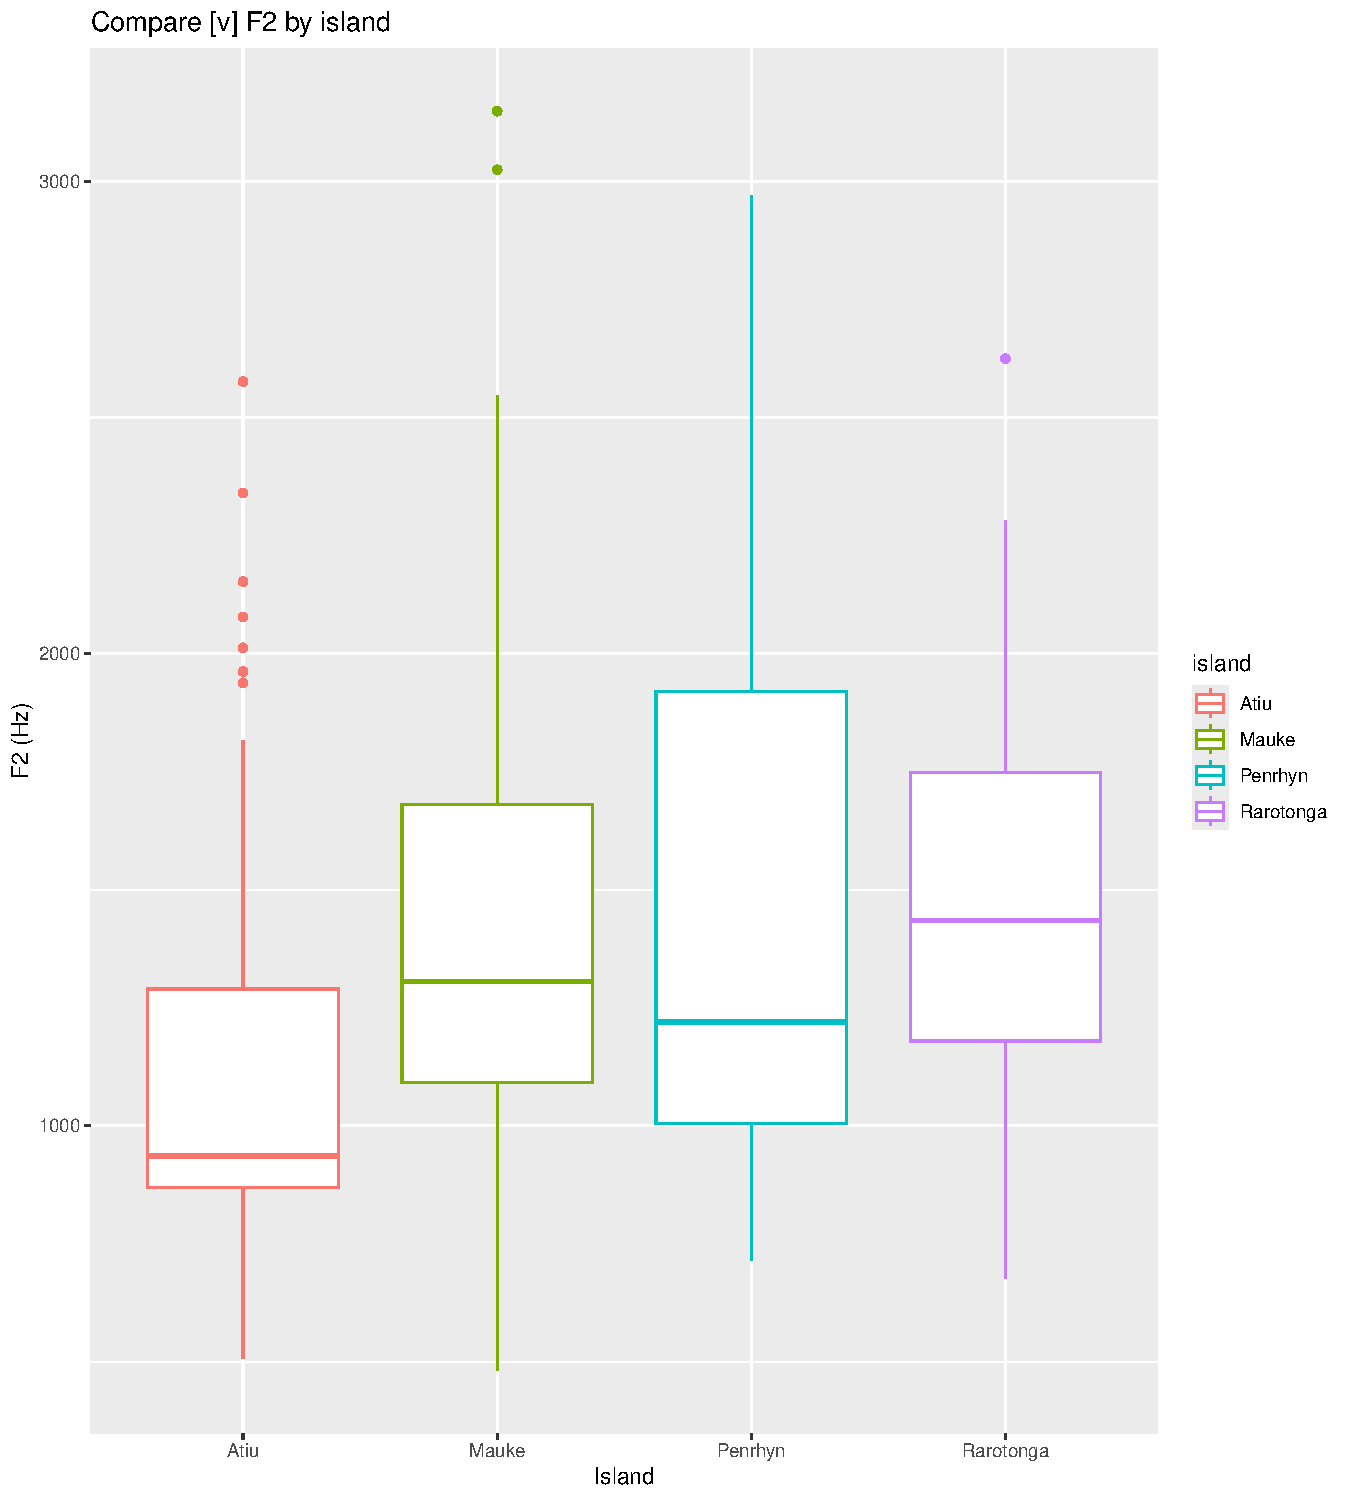
\includegraphics[width=2700px]{D2_CIM_files/figure-latex/print-f2-plot-1} \caption{ }\label{fig:print-f2-plot}
\end{figure}

From looking at the f2 boxplot, it's clear that Atiu has the lowest mean f2. \textbf{CONTINUE???}

\begin{verbatim}
## Linear mixed model fit by REML. t-tests use Satterthwaite's method [
## lmerModLmerTest]
## Formula: f2 ~ island + (1 | speaker) + (1 | word)
##    Data: tidy_f2
## 
## REML criterion at convergence: 13277
## 
## Scaled residuals: 
##     Min      1Q  Median      3Q     Max 
## -2.1832 -0.6452 -0.1646  0.5206  4.0860 
## 
## Random effects:
##  Groups   Name        Variance Std.Dev.
##  word     (Intercept)  37558   193.80  
##  speaker  (Intercept)   4625    68.01  
##  Residual             155390   394.20  
## Number of obs: 894, groups:  word, 145; speaker, 11
## 
## Fixed effects:
##                 Estimate Std. Error       df t value Pr(>|t|)    
## (Intercept)     1142.411     83.412    5.643  13.696 1.52e-05 ***
## islandMauke      297.881     90.354    4.946   3.297  0.02190 *  
## islandPenrhyn    384.930    111.231    4.466   3.461  0.02162 *  
## islandRarotonga  389.099     94.770    6.027   4.106  0.00626 ** 
## ---
## Signif. codes:  0 '***' 0.001 '**' 0.01 '*' 0.05 '.' 0.1 ' ' 1
## 
## Correlation of Fixed Effects:
##             (Intr) islndM islndP
## islandMauke -0.862              
## islndPnrhyn -0.703  0.648       
## islandRrtng -0.829  0.769  0.626
\end{verbatim}

\subsection{5.1 Data analysis}\label{data-analysis}

I used r cite\_r(``r-references.bib'') for all my analyses.

\section{6.0 Conclusion}\label{conclusion}

???fill in

\section{References}\label{references}

\setlength{\parindent}{-0.5in}
\setlength{\leftskip}{0.5in}


\clearpage
\renewcommand{\listfigurename}{Figure captions}

\clearpage
\renewcommand{\listtablename}{Table captions}


\end{document}
